% https://es.overleaf.com/latex/templates/project-report/jpzczmpsdzwm

%%% Preamble
\documentclass[paper=leter, fontsize=11pt]{scrartcl}
\usepackage[utf8]{inputenc}
\usepackage[spanish,mexico]{babel}
\usepackage[T1]{fontenc}    % use 8-bit T1 fonts
\usepackage{lmodern}
\usepackage{hyperref}       % hyperlinks
\usepackage{lipsum}
\usepackage[square,numbers]{natbib}

\usepackage[protrusion=true,expansion=true]{microtype}	
\usepackage{amsmath,amsfonts,amsthm} % Math packages
\usepackage[pdftex]{graphicx}
\usepackage{url}
% https://tex.stackexchange.com/a/3785
\usepackage{breqn}
 
\usepackage{booktabs}
\usepackage[table,xcdraw]{xcolor}

\usepackage{tikz}
\usetikzlibrary{positioning,matrix, arrows.meta}

\usepackage{caption} 
\usepackage{subcaption}

\usepackage{multirow}

\usepackage{listings}
\lstdefinestyle{mystyle}{ 
    language=R,
    basicstyle=\ttfamily\footnotesize,
    breakatwhitespace=false,         
    breaklines=true,                 
    captionpos=b,                    
    keepspaces=true,                 
    numbers=left,                    
    numbersep=5pt,                  
    showspaces=false,                
    showstringspaces=false,
    showtabs=false,                  
    tabsize=2
}

\lstset{style=mystyle}
\renewcommand{\lstlistingname}{Código}


\selectlanguage{spanish}
\usepackage[spanish,onelanguage,ruled]{algorithm2e}


%%% Custom sectioning
\usepackage{sectsty}
\allsectionsfont{\centering \normalfont\scshape}


%%% Custom headers/footers (fancyhdr package)
\usepackage{fancyhdr}
\pagestyle{fancyplain}
\fancyhead{}											% No page header
\fancyfoot[L]{}											% Empty 
\fancyfoot[C]{}											% Empty
\fancyfoot[R]{\thepage}									% Pagenumbering
\renewcommand{\headrulewidth}{0pt}			% Remove header underlines
\renewcommand{\footrulewidth}{0pt}				% Remove footer underlines
\setlength{\headheight}{13.6pt}


%%% Equation and float numbering
%\numberwithin{equation}{section}		    % Equationnumbering: section.eq#
%\numberwithin{figure}{section}			    % Figurenumbering: section.fig#
%\numberwithin{table}{section}				% Tablenumbering: section.tab#


%%% Maketitle metadata
\newcommand{\horrule}[1]{\rule{\linewidth}{#1}} 	% Horizontal rule

%%% https://tex.stackexchange.com/a/118217
\usepackage{mathtools}
\DeclarePairedDelimiter\ceil{\lceil}{\rceil}
\DeclarePairedDelimiter\floor{\lfloor}{\rfloor}

\title{
		%\vspace{-1in} 	
		\usefont{OT1}{bch}{b}{n}
		\normalfont \normalsize \textsc{Posgrado de Ingeniería de Sistemas} \\ [25pt]
		\horrule{0.5pt} \\[0.4cm]
		\huge Convolución y Chi cuadrada \\
		\horrule{2pt} \\[0.5cm]
}
\author{
		\normalfont 								\normalsize
        Alberto Benavides\\[-3pt]		\normalsize
        \today
}
\date{}


%%% Begin document
\begin{document} 
\maketitle

\section{Sobre los datos}
Los datos para esta tarea provienen del tema de tesis que actualmente trabajo: relación entre contaminantes y enfermedades en el \emph{área metropolitana de Monterrey} (AMM). Los datos de los contaminantes fueron obtenidos del SIMA \citep{aireNL}, mientras que los datos de las enfermedades provienen de la página de la Secretaría de Salud de Méxito \citep{egresos}. Los datos de contaminantes fueron tomados cada segundo por las distintas trece estaciones de monitoreo ambiental ubicadas en el AAM e incluyen concentraciones de algunos contaminantes, de los que se destacan los que tienen tamaños de partículas de $10$ PM medidas en $\mu$g $/$ m$^3$, en tanto que los datos de las enfermedades contienen información sobre la edad, género, talla, enfermedad y, dato de principal interés para esta tarea, la fecha en la que se dio la consulta de cada caso.

\section{Preprocesamiento de los datos}
A ambos conjuntos de datos se les eliminaron las inconsistencias como valores fuera de rangos permitidos o la ausencia de valores, posteriormente se obtuvieron sólo concentraciones de contaminantes y consultas del año 2017 por ser el año en que se hallan datos más completos. Posteriormente, se agruparon estos datos semanalmente, obteniendo el promedio semanal de las concentraciones de partículas de $10$ PM y la suma de todos los casos de consultas registradas, ambos datos mostrados en la figura \ref{datos} (p. \pageref{datos}).

\begin{figure}
  \begin{subfigure}{.5\textwidth}
      \centering
      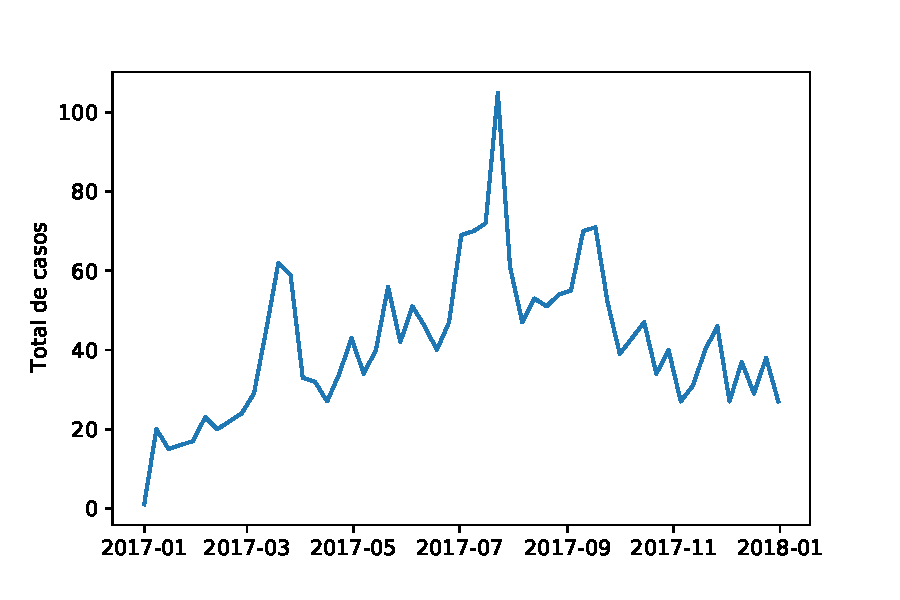
\includegraphics[scale=0.4]{2017_ingresos_semana.pdf}
      \caption{Casos.}
  \end{subfigure}
  \begin{subfigure}{0.5\textwidth}
      \centering
      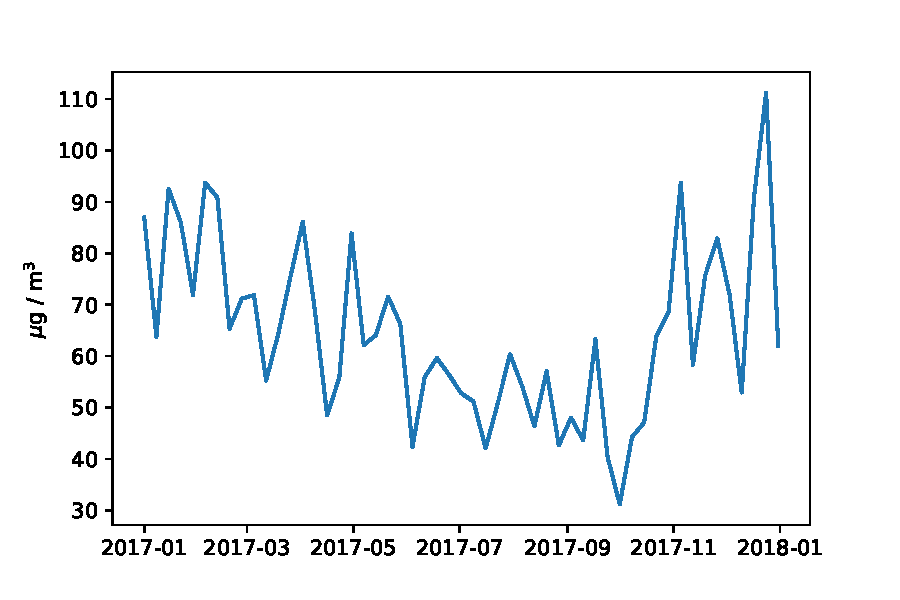
\includegraphics[scale=0.4]{2017_PM10_semana.pdf}
      \caption{Partículas de $10$ PM.}
  \end{subfigure}
  \caption{Series de tiempo de casos registrados de enfermedades y concentraciones de partículas de $10$ PM en el AMM durante 2017.}
  \label{datos}
\end{figure}

Una práctica común para comparar series de tiempo es normalizarlas y diferenciarlas mediante la resta de cada valor, menos su valor en una unidad de tiempo anterior, lo que hace que la serie de tiempo resultante tenga valores en torno a cero con valores de $[-1, 1]$, como puede verse en la figura \ref{diff} (p. \pageref{diff}).

\begin{figure}
    \centering
    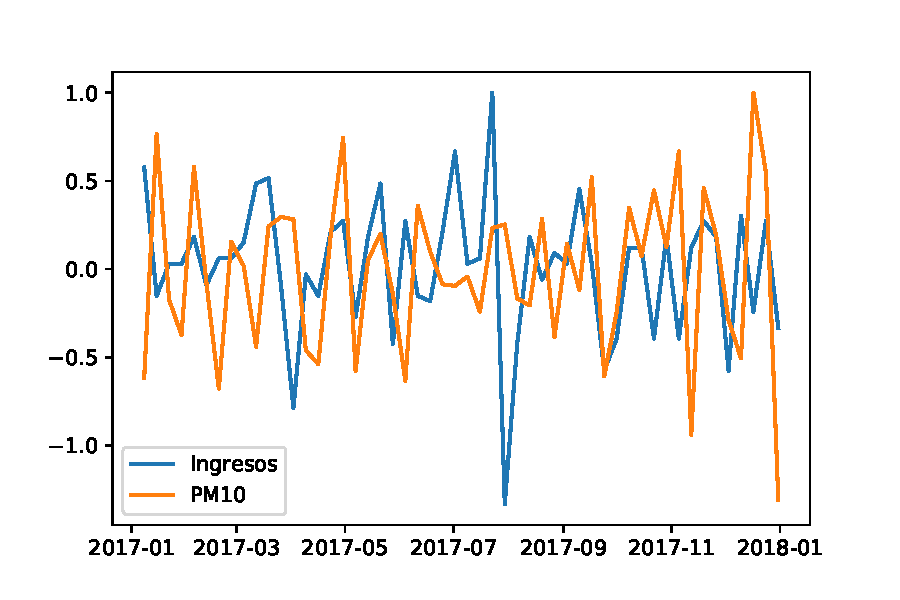
\includegraphics{2017_ingresos_PM10_diff_semana.pdf}
  \caption{Series de tiempo diferenciadas de casos registrados de enfermedades y concentraciones de partículas de $10$ PM en el AMM durante 2017.}
  \label{diff}
\end{figure}

\section{Chi cuadrada}

La prueba de Chi cuadrada tiene dos usos principales: Determinar la independencia entre conjuntos de datos y conocer si valores observados son similares a valores esperados. En este caso, se utiliza la prueba de Chi cuadrada para determinar si los valores diferenciados y normalizados de los contaminantes son independientes de los de las consultas de las enfermedades registradas y, también, si los casos registrados observados son similares a los esperados, tomados estos últimos como las concentraciones en promedio de las partículas de $10$ PM. 

Para el caso de la independencia, la hipótesis nula es que ambas variables son independientes. El $p$-valor obtenido es $1$ por lo que se acepta la hipótesis nula. Mientras que para el grado de similitud, la hipótesis nula es que los valores observados y esperados no tienen diferencia, pero ésta hipótesis se rechaza dado que el $p$-valor $= 6.07 \times 10 ^{-175}$.

\section{Convolución}

Una convolución muestra la distribución de probabilidad $Z$ de la suma de dos variables aleatorias $X$ y $Y$ tal que $P(Z = j) = \sum_{i =
-\infty}^\infty P(X = i) \times P(Y = j - i)$. Para el caso discreto, esto se puede calcular como $f_c(i) = \sum_j f_1(j) \times f_2(i - j)$, en tanto para el continuo se tiene $(f \ast g)(z) = \int_{-\infty}^\infty f(z - x) \times g(x) \text{d} x$. Este concepto de convolución también se puede utilizar para conocer las interacciones entre dos series de tiempo de modo que se obtiene el grado de relación de una respecto a la otra desfasada en el tiempo. La convolución de las series de tiempo diferenciadas puede verse en la figura \ref{conv} (p. \pageref{conv}).

\begin{figure}
  \centering
  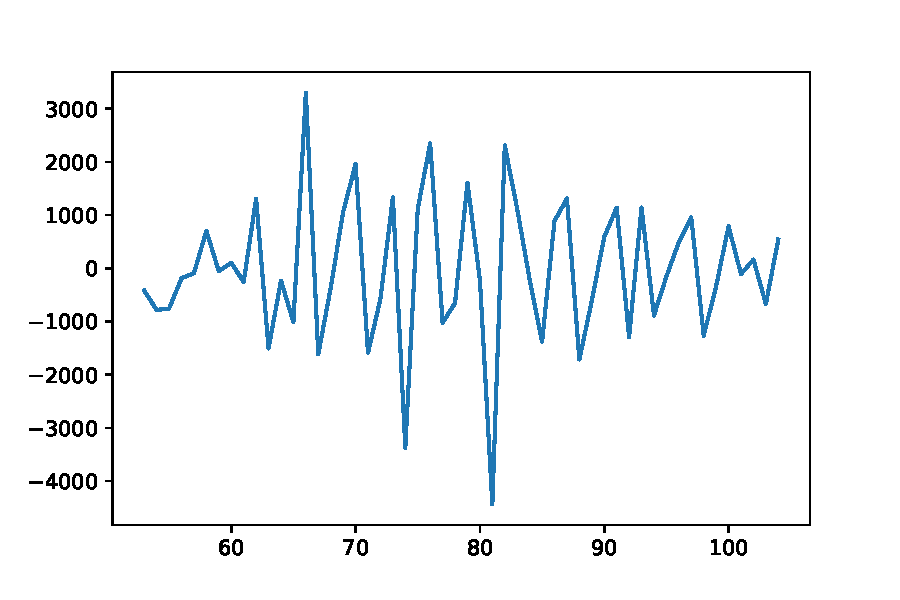
\includegraphics{2017_ingre_PM10_conv_semana.pdf}
\caption{Convolución de las series de tiempo diferenciadas de casos registrados de enfermedades y concentraciones de partículas de $10$ PM en el AMM durante 2017.}
\label{conv}
\end{figure}


\bibliographystyle{plainnat}
\bibliography{Biblio}

\end{document}